\documentclass[discrete.tex]{subfiles}

\begin{document}
    \section{Задача коммивояжера. Метод ветвей и границ}

    \begin{task}[Задача коммивояжера]
        Дали $n$ городов (вершины графа), между городами есть какие-то дороги, 
        по каждой можно проехать за какое-то фикс. время (вес ребра). 
        Необходимо найти самый дешевый маршрут, проходящий через все города
        только один раз (тут возможны варианты) с последующим возвратом в 
        исходный город.\\
        \\
        Очевидно наивное решение за $O(n!)$, что неприменимо на практике
    \end{task}

    \begin{Definition}[метод ветвей и границ]
        Метод для решения различных задач оптимизации. В отличии от полного 
        перебора отсеивает подмножества допустимых решений. 
        \[f(x) \text{ - ф-я, которую мы хотим минимизировать}\]
        \[D \text{ - мн-во допустимых решений}\]
        Ветвление - разбиение мн-ва допустимых решений на подмн-ва\\
        Ветвление можно рекурсивно применять к подобластям. Полученные 
        подобласти образуют дерево поиска или дерево ветвей и границ. \\
        Процедура нахождения оценки (границы) заключается в поиске верхних и 
        нижних границ для решения задачи на подобласти.\\
        В основе метода лежит след. идея, если нижняя граница на подобласти 
        $A$ больше, чем верхняя граница на ранее просмотренной $B$, то 
        $A$ может быть исключена из дальнейшего рассмотрения.
        Обычно минимальную из полученных верхних оценок записывают
        в глобальную переменную $M$
    \end{Definition}

    \begin{task}[решение ]
        Зафиксируем какую-нибудь вершину, очевидно, что выбор не важен\\
        Мы можем начать строить дерево путей. 
        Будем поддерживать абсолютный минимум в переменной M.
        Если мы дошли до листа, то обновляем минимум. Дальше, делая обход, 
        мы можем сделать оценку, обозначим за S.
        Допустим, мы прошли какую-то часть пути (часть ветви),
        обозначим 
        сумму весов на ней за $W$, оставшийся граф значим за $G'$
        К оценке добавим самое короткое ребро (r) из вершины, на которой 
        мы остановились до $G'$ и вес минимального остовного дерева на $G'$.
        Таким образом, мы оценили снизу решение задачи на этой ветви. 
        \[S = W + \omega(r) + \omega(MST(G'))\]
        Если S > M, то можно дальше не спускаться вниз и не рассматривать этот 
        путь дальше, он гарантированно не будет оптимальнее.
        \begin{figure}[H]
            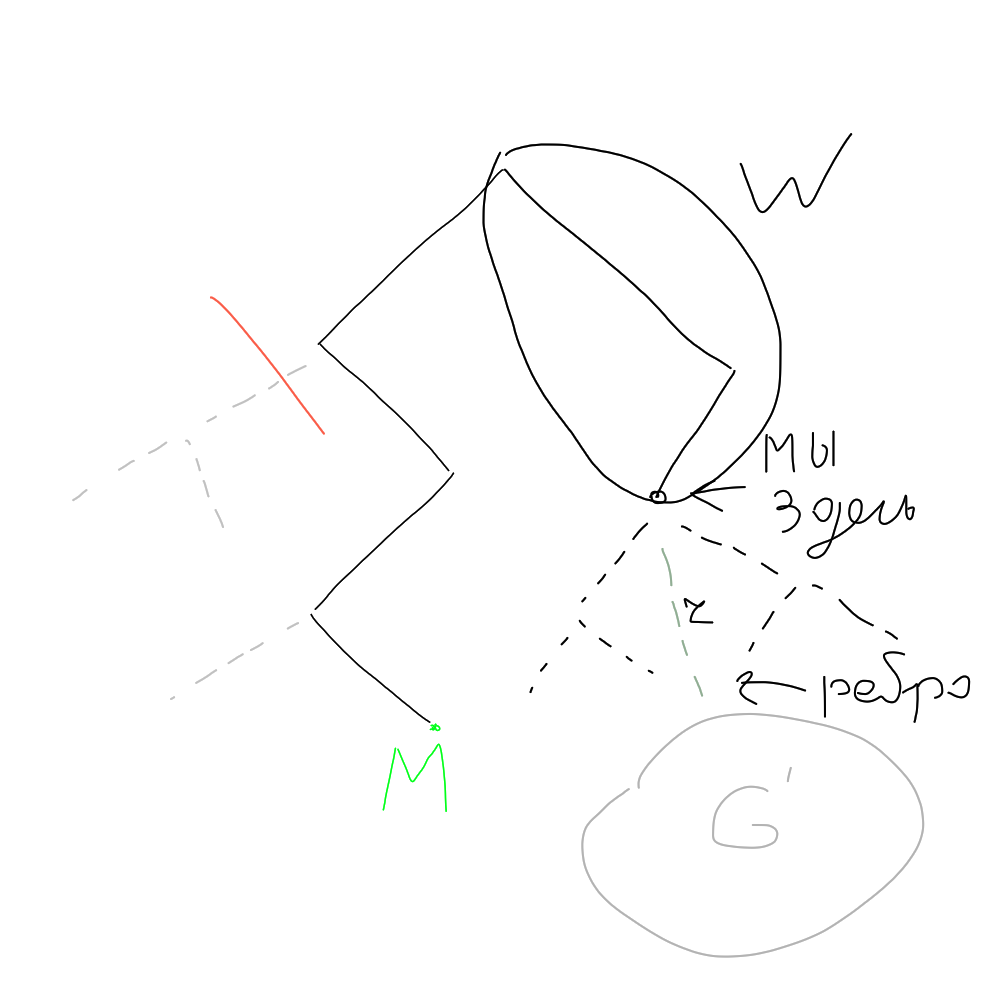
\includegraphics[width=7cm]{pics/53_1.png}
            \centering
        \end{figure}
        \begin{figure}[H]
            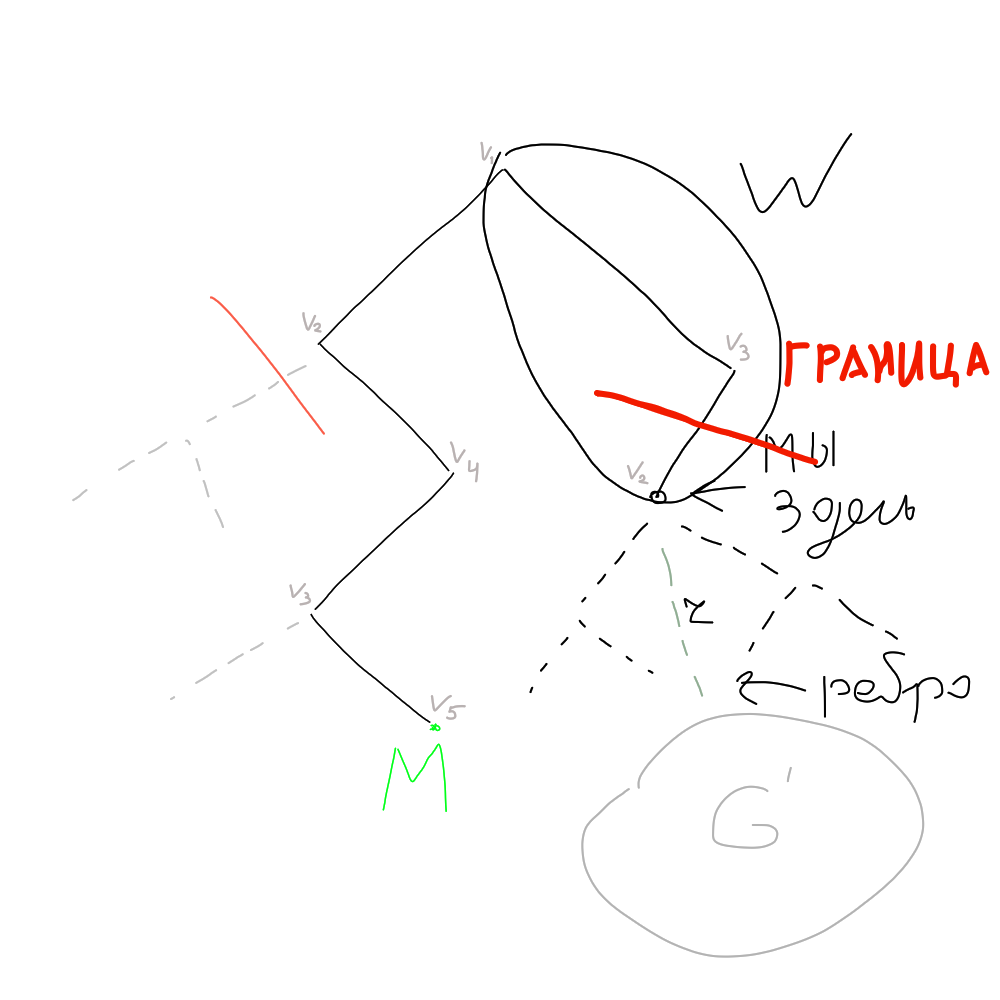
\includegraphics[width=7cm]{pics/53_2.png}
            \centering
        \end{figure}
        
        В качестве нижней оценки можно использовать и более хитрые функции. А 
        вообще достоинством $MST$ является быстрое получение ответа, хотя оценка 
        и немного грубовата.
    \end{task}
    \newpage
\end{document}
